% \begin{table}[H]
%     \centering
%     \begin{tabular}{|c|c|c|c|c|c|c|}
%         \hline
%         \textbf{Agent} & \textbf{Exploration} & \textbf{n Step} & \textbf{Distributional} & \textbf{SAD} & \textbf{Score(Std.dev)} \\ \hline
%         Simple DQN     & $\epsilon$-Greedy    & 1               & No                      & No           & 0.502(0.7)              \\ \hline
%         Rainbow        & Noisy Networks       & 1               & Yes                     & No           & 3.26(1.07)              \\ \hline
%         Rainbow        & Noisy Networks       & 3               & Yes                     & No           & 1.01(1.48)              \\ \hline
%         Rainbow        & Noisy Networks       & 5               & Yes                     & No           & 3.17(1.47)              \\ \hline
%         Distributed    & $\epsilon$-Greedy    & 1               & Yes                     & No           & 2.47(1.35)              \\ \hline
%         SAD Agent      & $\epsilon$-Greedy    & 1               & Yes                     & Yes          & 2.69(0.98)              \\ \hline
%         SAD Agent      & $\epsilon$-Greedy    & 3               & Yes                     & Yes          & 2.64(0.72)              \\ \hline
%     \end{tabular}
%     \caption{Performance of learning agents in Self-Play}
%     \label{tab:algorithm_comparison}
% \end{table}

\begin{table*}
  \caption{Performance of learning agents in Self-Play}
  \label{tab:sp_performance}
  \begin{tabular}{|c|c|c|c|c|c|c|}
    \toprule
    \textbf{Agent} & \textbf{Exploration} & \textbf{n Step} & \textbf{Distributional} & \textbf{SAD} & \textbf{Score(std.dev)} \\
    \midrule
    Simple DQN & $\epsilon$-Greedy & 1 & No & No & 0.502(0.7) \\
    Rainbow & Noisy Networks & 1 & Yes & No & 3.26(1.07) \\
    Rainbow & Noisy Networks & 3 & Yes & No & 1.01(1.48) \\
    Rainbow & Noisy Networks & 5 & Yes & No & 3.17(1.47) \\
    Distributed & $\epsilon$-Greedy & 1 & Yes & No & 2.78(1.05) \\
    SAD Agent & $\epsilon$-Greedy & 1 & Yes & Yes & 2.69(0.98) \\
    SAD Agent & $\epsilon$-Greedy & 3 & Yes & Yes & 2.64(0.72) \\   
  \bottomrule
\end{tabular}
\end{table*}

\begin{figure*}[h]
 
  \centering
  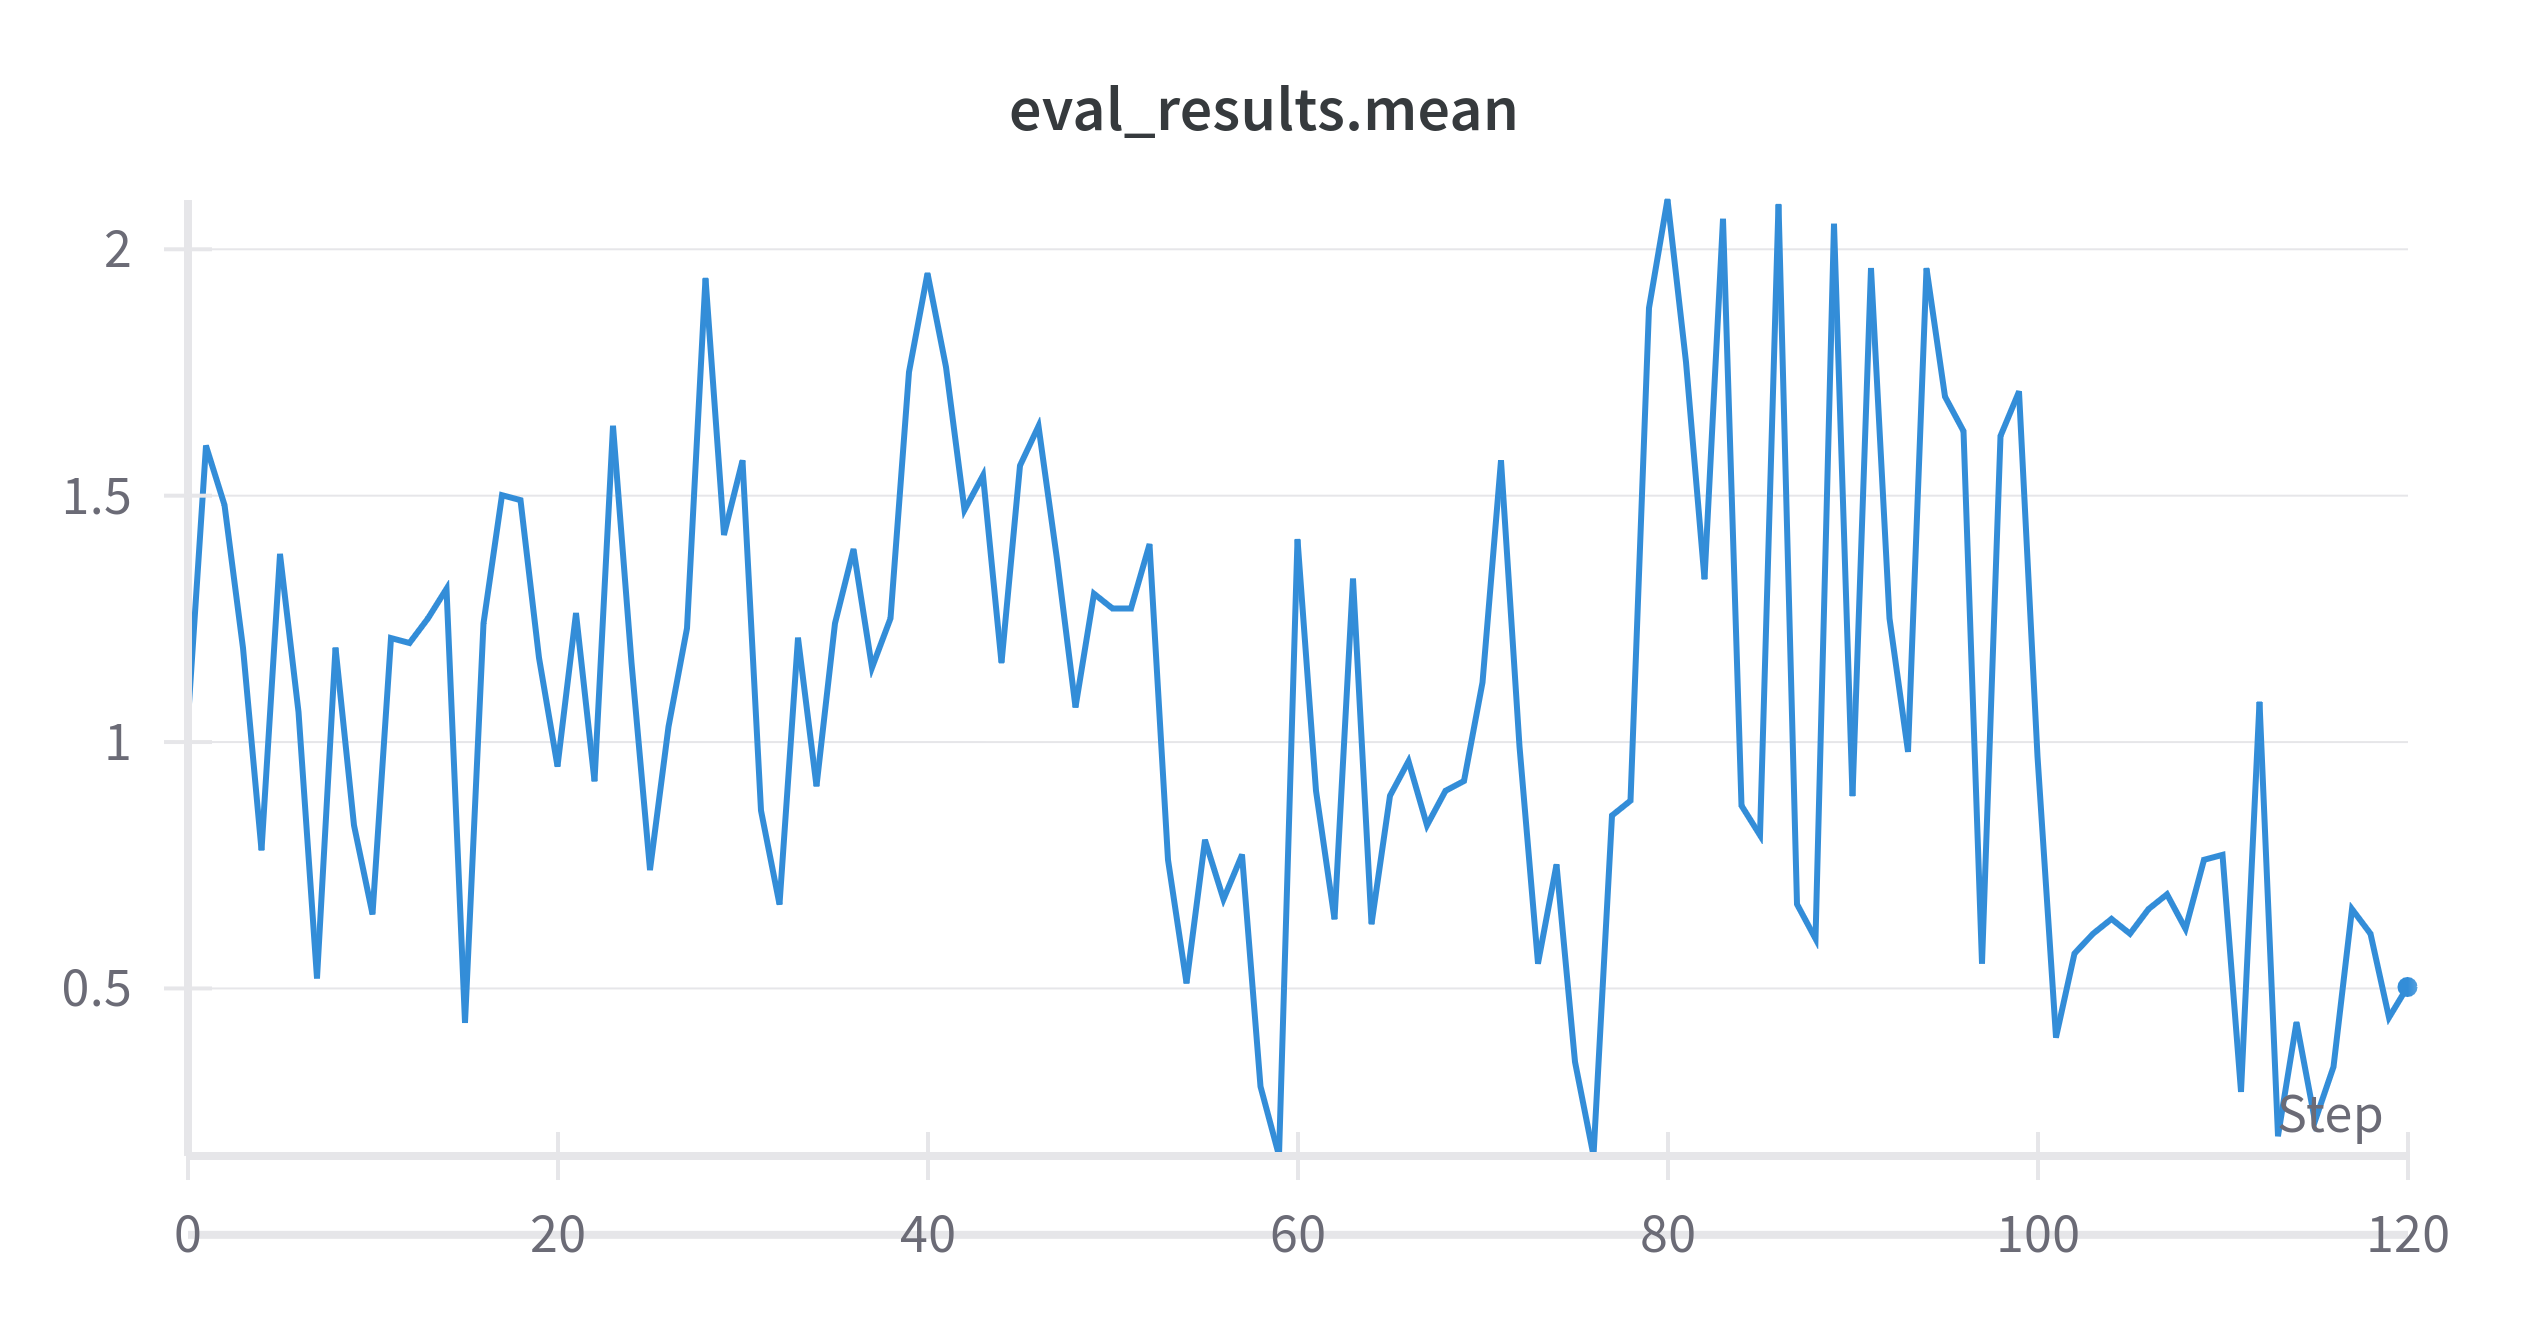
\includegraphics[width=\linewidth]{results/IQL.png}
  \caption{
    Training curve for Simple DQN Agent
  }
  \Description{Training curve for Simple DQN Agent}
  \label{fig:dqn}
\end{figure*}

\begin{figure*}[h]
  \centering
  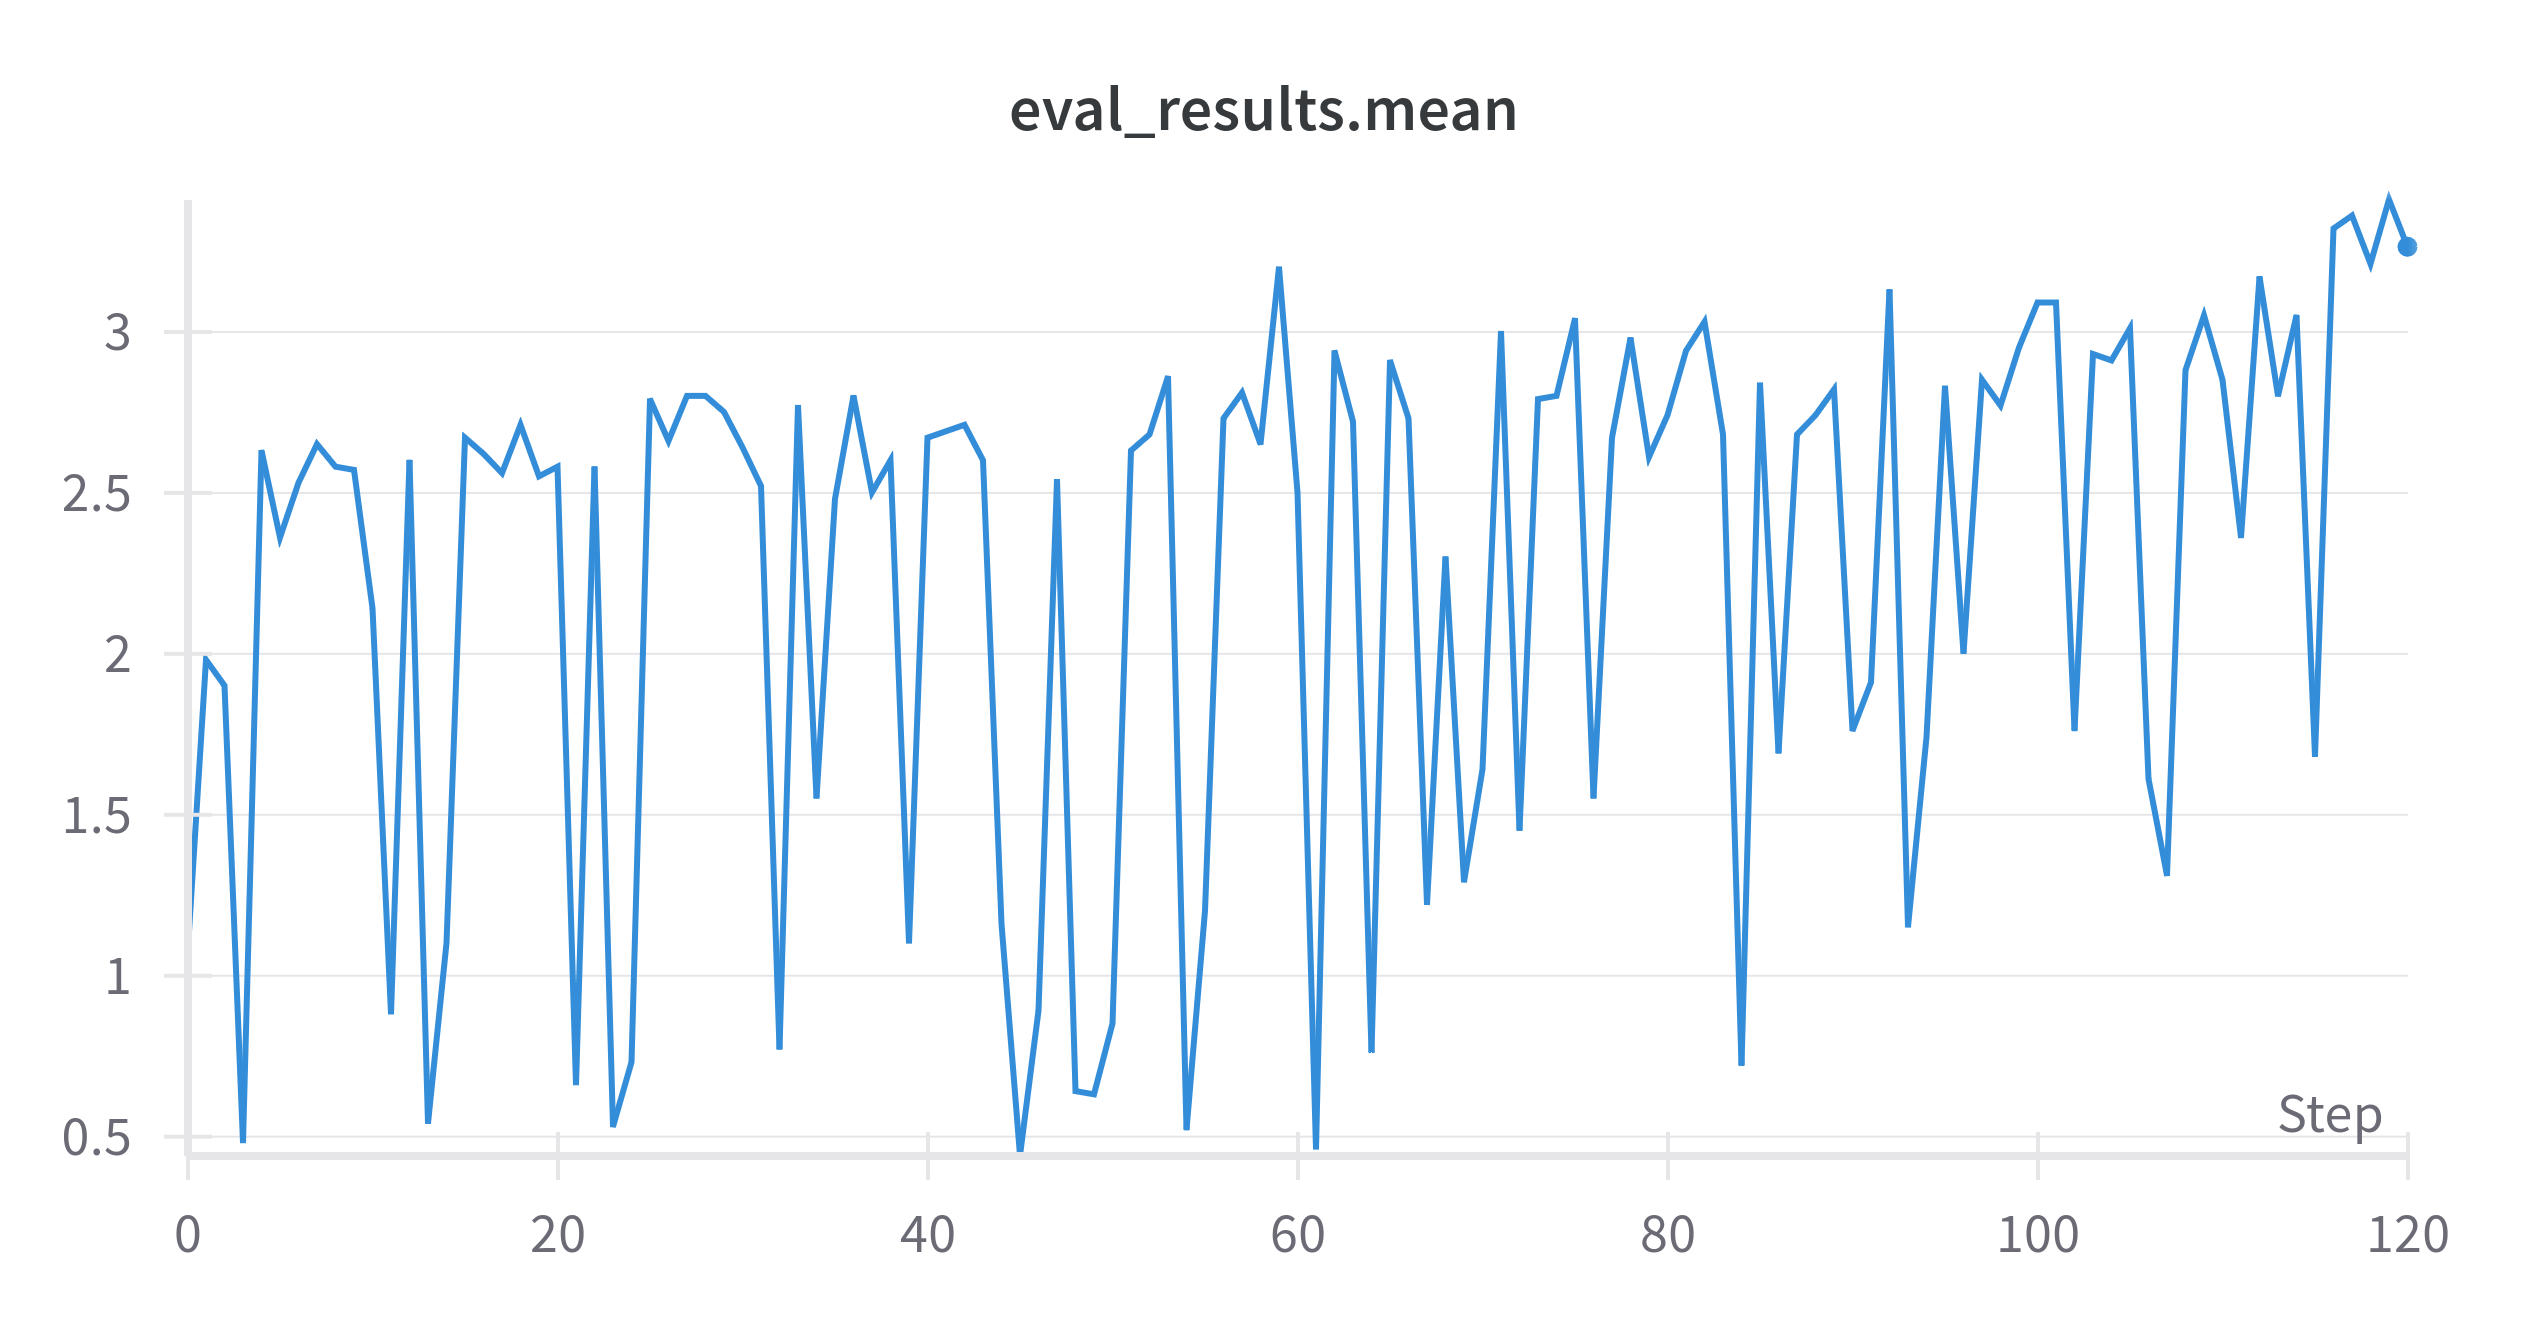
\includegraphics[width=\linewidth]{results/RAINBOW-mean.png}
  \caption{
    Training curve for Rainbow Agent
  }
  \Description{Training curve for Rainbow Agent}
  \label{fig:rainbow}
\end{figure*}

% \begin{figure*}[h]
%   \centering
%   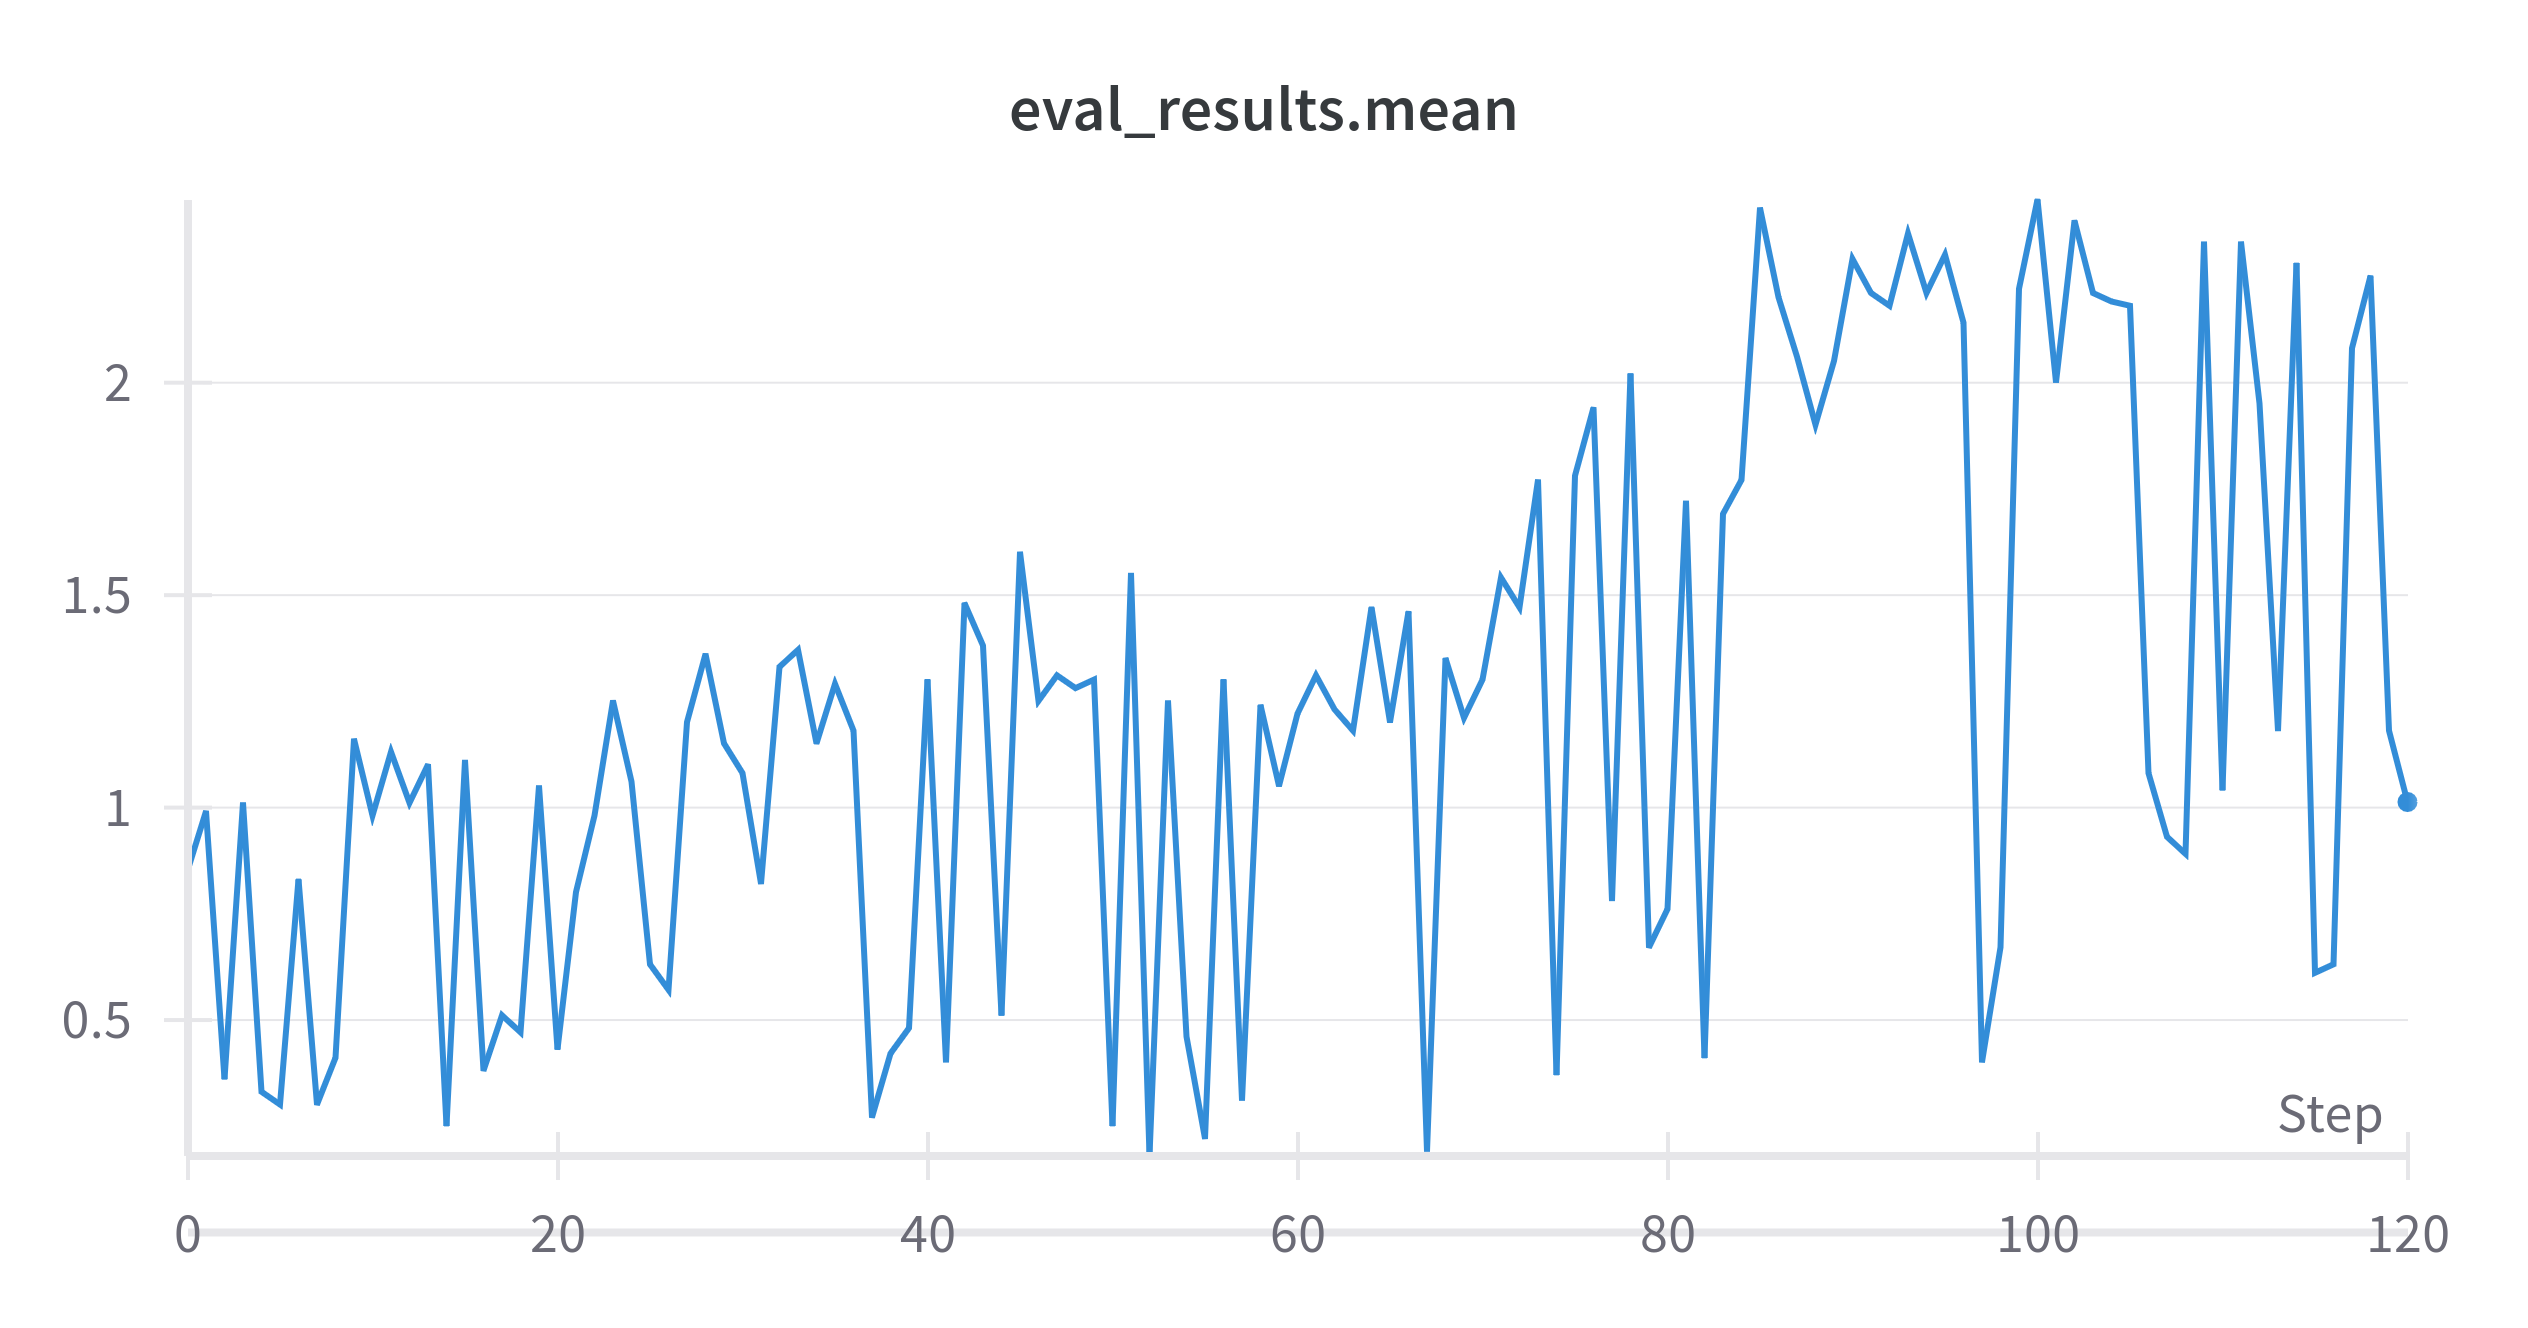
\includegraphics[width=\linewidth]{results/RAINBOW-3-mean.png}
%   \caption{
%     Training curve for Rainbow-3 Agent
%   }
%   \Description{Training curve for Rainbow-3 Agent}
% \end{figure*}

% \begin{figure*}[h]
%   \centering
%   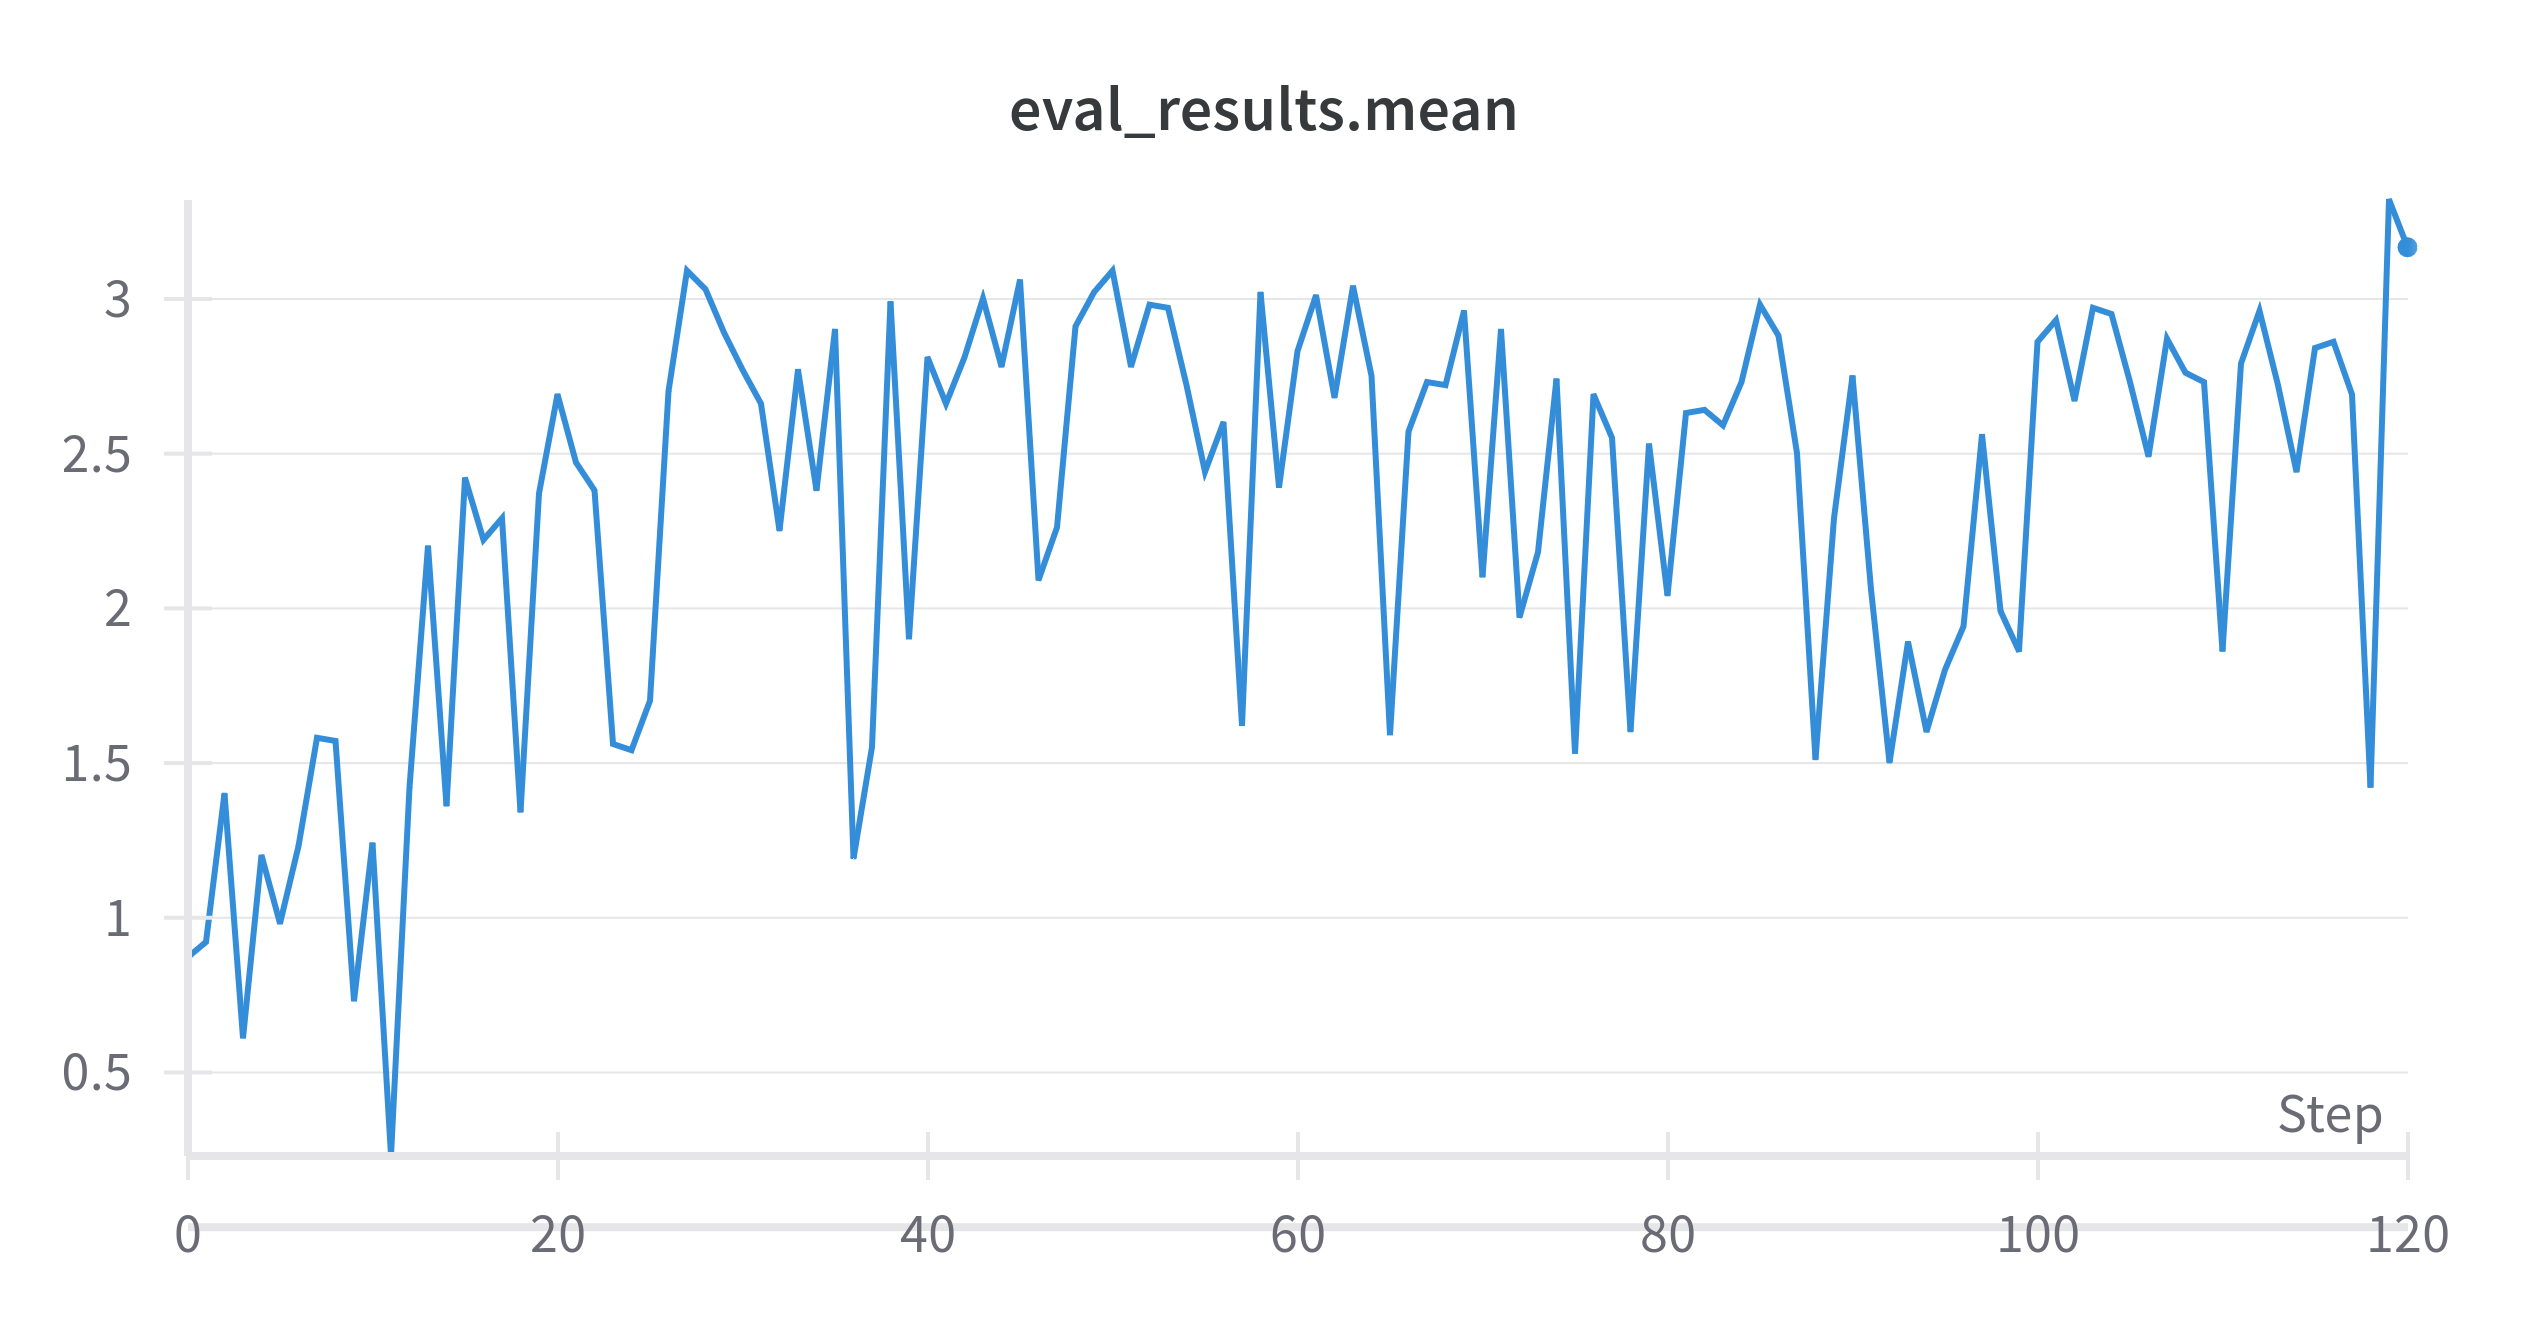
\includegraphics[width=\linewidth]{results/RAINBOW-5-mean.png}
%   \caption{
%     Training curve for Rainbow-5 Agent
%   }
%   \Description{Training curve for Rainbow-5 Agent}
% \end{figure*}


% \begin{figure*}[h]
%   \centering
%   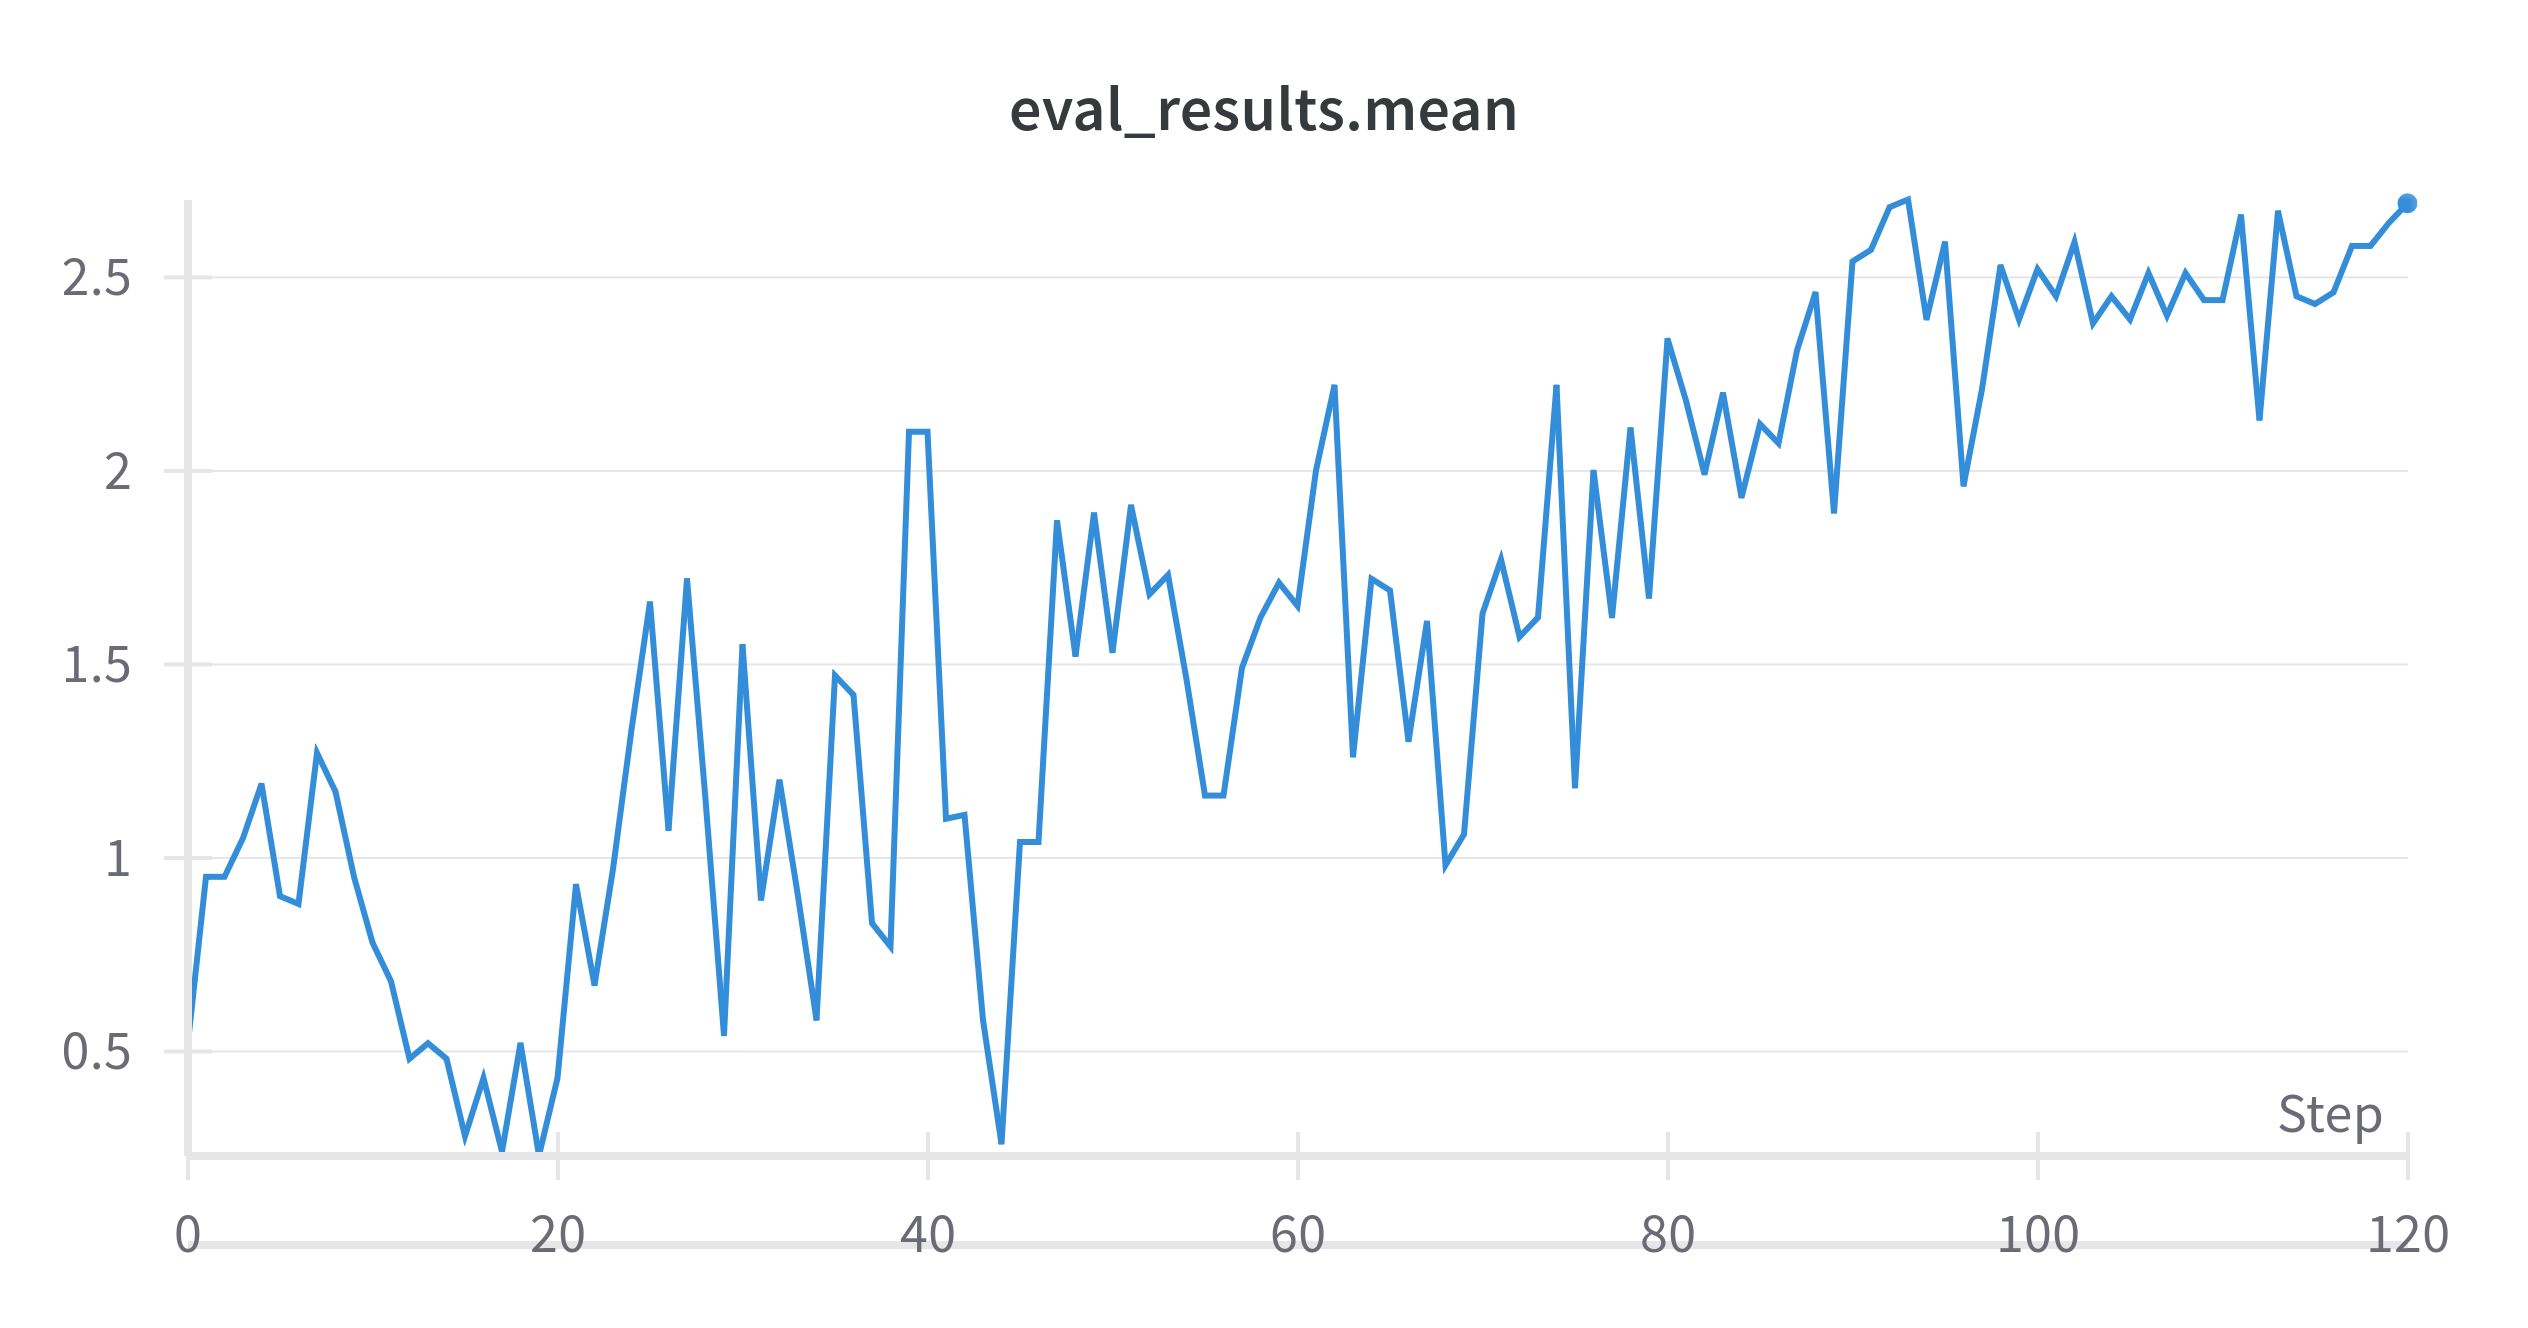
\includegraphics[width=\linewidth]{results/SAD-mean.png}
%   \caption{
%     Training curve for SAD Agent
%   }
%   \Description{Training curve for SAD Agent}
% \end{figure*}

\begin{figure*}[h]
  \centering
  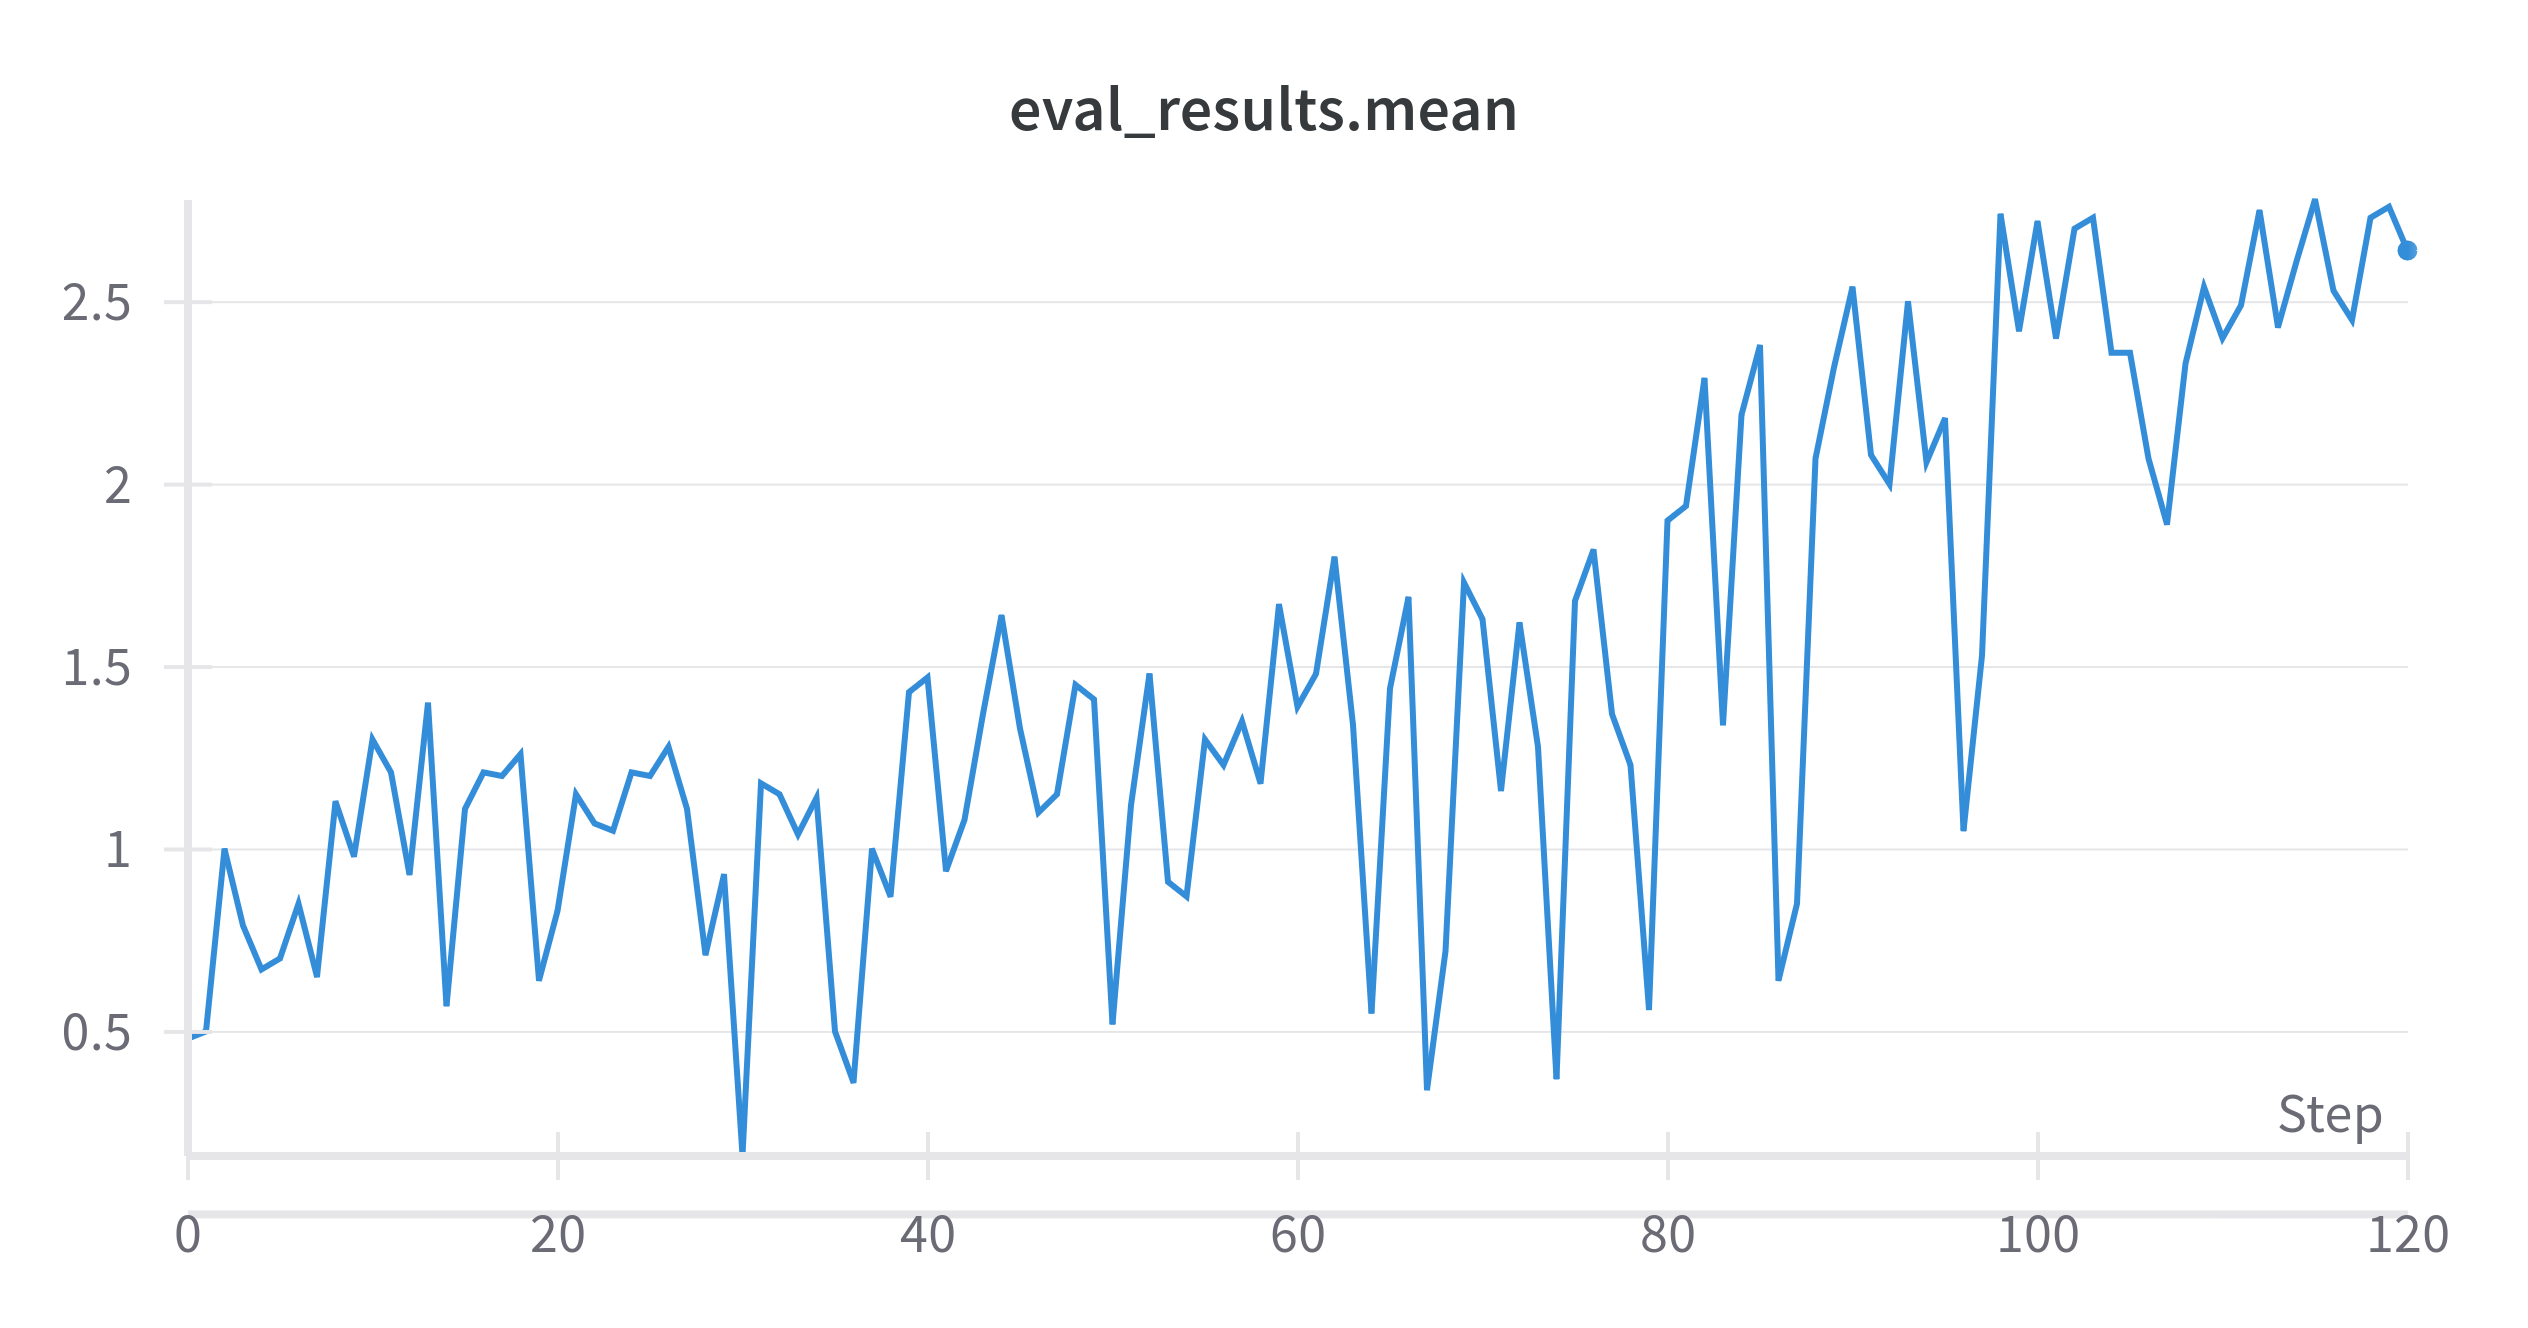
\includegraphics[width=\linewidth]{results/SAD-3-mean.png}
  \caption{
    Training curve for SAD-3 Agent
  }
  \Description{Training curve for SAD-3 Agent}
  \label{fig:sad3}
\end{figure*}